% 官方要求：
% 1.整体机械结构设计/核心结构设计说明
% 2.工艺选择
% 3.传感器的设计安装、电路板的固定及走线情况
% 4.核心零件的有限元分析、静力学分析

\subsection{整体机械结构设计}

无人机的整体机械结构在大体上可以分为飞行平台与发射系统两个部分，飞行平台是无人机最基础的功能载体，其结构刚度与轻量化直接决定飞行性能；发射系统则决定空中机器人的攻击上限。两个部分协同配合，共同构成完整的空中机器人机械系统。各部分细分结构关系见\tabref{tab:无人机机械结构总览}所示。

\begin{table}[hbtp!]
    \centering
    \begin{tabular}{ m{3cm} m{4cm} m{6cm} }
    \toprule
    一级分类 & 二级分类 & 三级分类 \\
    \midrule
    \multirow{4}*{飞行平台}
       & \multirow{4}*{机身整体} & 机身中心 \\
       &  & 机臂（可折叠） \\
       &  & 脚架（分体式） \\
       &  & 弹仓 \\
    \midrule
    \multirow{2}*{飞行平台}
       & 动力系统 & 桨叶 \\
       &  & 旋翼电机 \\
    \midrule
    飞行平台 & GPS平台 & 雷达、激光检测模块安装位 \\
    \midrule
    \multirow{2}*{飞行平台}
       & \multirow{2}*{桨保} & 框架（分体式） \\
       &  & 覆盖网 \\
    \midrule
    \multirow{3}*{发射系统}
       & \multirow{3}*{云台} & 弹丸链路 \\
       &  & 发射机构 \\
       &  & 元件布局 \\
    \midrule
    发射系统 & 拨盘 & 供弹拨盘 \\
    \midrule
    发射系统 & 云台架 & 长脖子吊装结构 \\
    \bottomrule
    \end{tabular}
    \caption{无人机机械结构总览}
    \label{tab:无人机机械结构总览}
\end{table}

% 图片占位：整体结构图
% \begin{figure}[hbt!]
%     \centering
%     \includegraphics[width=0.8\columnwidth]{figure/4_详细设计/机械结构设计/整体结构图.png}
%     \caption{无人机整体结构}
%     \label{fig:无人机整体结构}
% \end{figure}

\subsubsection{飞行平台机械结构设计}

飞行是一台无人机最基础的功能，飞行平台的结构是无人机最重要的结构。对它的要求是：
\begin{enumerate}
    \item 整体刚度大，能够减少无人机在飞行过程中的震动，并且在发生意外坠机时能保证不发生严重破坏。
    \item 质量轻，轻量化设计理念贯穿整个无人机机械设计过程，飞行平台是减重的大头。
\end{enumerate}

无人机在飞行时会产生很多高频震动，如果机身设计不稳定或刚度不够会极大程度影响飞行平稳性和飞机的操控性，进而影响发射系统，所以优秀的飞行平台设计是赛场上空中机器人发挥优秀的基础。接下来依次介绍飞行平台各个部分的设计以及之间的联系。

% 图片占位：飞行平台装配图
% \begin{figure}[hbt!]
%     \centering
%     \includegraphics[width=0.8\columnwidth]{figure/4_详细设计/机械结构设计/飞行平台装配.png}
%     \caption{飞行平台装配}
%     \label{fig:飞行平台装配}
% \end{figure}

\paragraph{机身中心结构}

机身的中心结构是整个飞行平台的中心，所有其他的结构都固定在机身中心板上，向四周伸出四根机臂，下面接脚架，上面接弹仓，而且飞控、主控等电子元件也固定在其中。它的组成结构很简单，就是由上下两层碳板中间加铝柱构成。

因为要与机身其他机构连接所以做了很多固定的孔位，并在空白处做大量镂空减重。所以从中心板的孔位布局能够看出飞行平台的布局方式。以中心下板为例说明孔位功能：

% 图片占位：中心板孔位图
% \begin{figure}[hbt!]
%     \centering
%     \includegraphics[width=0.8\columnwidth]{figure/4_详细设计/机械结构设计/下中心板孔位.png}
%     \caption{下中心板孔位}
%     \label{fig:下中心板孔位}
% \end{figure}

蓝色圈1是机臂方管的固定孔，红圈2是脚架的固定孔，黄圈3是给分电板吊装预留的，绿圈4是云台架的固定孔位，5是留给弹仓波纹管的通道，周边是波纹管固定孔，其他孔位是上下两层中心板之间的加强铝柱孔。所以机身中心结构的设计重点是考虑整个飞行平台的布局，先把整机尺寸与各个部分的相对位置确定下来以后，中心机构自然就设计出来了。建议首先从飞机的功能出发，确定机臂大致尺寸、云台是否前置、脚架位置等因素，才能够把整机的布局确定。总的来说机身中心是整个飞行平台的固定点，所以中心板需要高强度的同时各元件布局也需要合理且紧凑。

\paragraph{机臂设计}

机臂是连接机身中心与旋翼电机的关键结构，需要承受飞行时的拉力与震动。今年的机臂在去年碳方管方案基础上新增了折叠功能，以满足检录收纳尺寸要求。

机臂选用$30\times30$、壁厚$1\mathrm{mm}$的碳方管。方管形变比圆管小，不需要调节桨平，还能在侧面镂空减重。方管机臂侧面的镂空采用拓扑方法，通过Altair inspire软件拓扑仿真后得出具体镂空形状，在保证强度的前提下实现最大程度的减重。

折叠机构是今年机臂设计的核心改动。机臂通过折叠座与机身中心板连接，展开后通过锁定机构固定，保证飞行时机臂的刚性与稳定性；折叠后机臂向机身内侧收拢，大幅减小整机尺寸，满足最大收纳尺寸的检录要求。折叠机构的设计需要兼顾展开锁定的可靠性与折叠操作的便捷性，确保赛场上能够快速部署。

% 图片占位：机臂折叠机构图
% \begin{figure}[hbt!]
%     \centering
%     \includegraphics[width=0.8\columnwidth]{figure/4_详细设计/机械结构设计/机臂折叠机构.png}
%     \caption{机臂折叠机构}
%     \label{fig:机臂折叠机构}
% \end{figure}

\paragraph{脚架结构设计}

无人机脚架的作用是支撑整架飞机，在迫降甚至坠机时是受力最大的结构，而且脚架离机身最远，最容易产生震动从而影响飞行效果，所以需要极高的稳定性与刚度。

今年采用分体式脚架设计，主要原因是为了配合机臂折叠需求，满足检录收纳尺寸限制。分体式脚架在折叠时可以拆卸或收拢，进一步减小整机收纳尺寸。

脚架尺寸最大的影响因素是云台，因为云台在脚架中间运动时很容易和脚架发生干涉，所以先定云台的活动范围，再定脚架的长度以及间距。脚架与机身中心下板连接处采用了快拆管夹转接件，方便拆卸，能快速处理脚架损坏。脚架下端加了横杆约束脚架的横向位移，形成更加稳定的三角形结构，在轻度坠机情况下仍能保证脚架主体结构的完整性。

% 图片占位：脚架结构图
% \begin{figure}[hbt!]
%     \centering
%     \includegraphics[width=0.8\columnwidth]{figure/4_详细设计/机械结构设计/脚架结构.png}
%     \caption{分体式脚架结构}
%     \label{fig:脚架结构}
% \end{figure}

\paragraph{弹仓设计}

弹仓设计首先考虑容量，本赛季允许最大发弹量750发。弹仓的尺寸和形状在很大程度上取决于上中心板的尺寸和电池的摆放位置。今年弹仓采用$0.5\mathrm{mm}$碳板制作，相比去年的$1\mathrm{mm}$碳板进一步减重，并在结构上加大镂空处理，在保证强度的前提下实现轻量化。弹仓位于上中心板上方，需要与电池、GPS平台等元件合理布局，避免干涉。

\subsubsection{GPS平台}

GPS平台是今年新增的结构模块，用于安装定位与感知传感器。GPS平台位于四个分体式桨保的正中间位置，处于机身顶部中心区域。

平台上主要安装两类传感器：
\begin{itemize}
    \item \textbf{Livox MID-360雷达}：采用纳米胶与电工胶将雷达直接粘贴在海绵垫上，这种减震方式效果最佳，既保证了雷达的稳定性，又不会产生过大的机械位移。雷达直接安装在GPS平台上。
    \item \textbf{激光检测模块}：安装在机身的长保护杆上，用于检测反无人机激光并触发规避机动。
\end{itemize}

GPS平台的设计需要考虑传感器的安装位置、减震效果以及与周边结构的避让关系。虽然激光检测模块的保护杆可能会对雷达产生轻微遮挡，但实际测试表明影响不大，不影响定位性能。

% 图片占位：GPS平台安装图
% \begin{figure}[hbt!]
%     \centering
%     \includegraphics[width=0.8\columnwidth]{figure/4_详细设计/机械结构设计/GPS平台.png}
%     \caption{GPS平台与传感器安装}
%     \label{fig:GPS平台}
% \end{figure}

\subsubsection{动力系统}

动力系统是无人机飞行的核心，直接决定飞行性能与续航能力。动力系统主要由旋翼电机与桨叶两部分组成。

\paragraph{旋翼电机}

本赛季采用好盈8100UL旋翼电机，该电机在25赛季中已得到广泛验证，性能稳定可靠。满载整机重量将近$18\mathrm{Kg}$，该电机毫无压力，温度正常，从没出现过热等异常情况。

\paragraph{桨叶}

配套使用好盈3098桨叶，30寸大桨叶带来以下优势：
\begin{itemize}
    \item 提升气动效率，增加续航时间
    \item 更大的桨叶能产生更大的总体升力，改善飞行稳定性和悬停性能
    \item 大桨叶具有更大的转动惯量，像陀螺仪一样有助于稳定无人机姿态
    \item 大桨叶在低转速下工作，产生的气流更平缓，湍流更少，悬停和低速飞行时更加平稳
\end{itemize}

但大桨叶也带来缺点：让整架无人机更难控制，任何微小的不平衡都会被放大，导致整机产生更剧烈的振动，严重影响飞控传感器的精度，所以对机身结构的稳定性要求更高。

\subsubsection{桨保设计}

桨保是覆盖在旋翼外围的保护结构，起到保护桨叶、防止异物进入以及安全防护的作用。今年采用分体式桨保设计，主要原因是配合机臂折叠需求，满足检录收纳尺寸限制。

桨保分为框架与覆盖网两部分。

\paragraph{框架}

分体式桨保框架相比去年的一体式桨保，最大的优势是便于维护。去年一体式桨保虽然刚度高、重量轻（约$1.2\mathrm{Kg}$），但飞机内部的中心板和飞控都被桨保覆盖，每次拔插飞控线或检修内部结构都需要拆卸桨保，维护非常不便。今年改为分体式后，每个桨保独立安装，维护时只需拆卸对应侧的桨保，大大提升了维护效率。

分体式桨保的缺点是重量略增（四个分体式桨保加起来约$1.6\mathrm{Kg}$），但换来的维护便捷性在实战中更有价值。

\paragraph{覆盖网}

覆盖网选用渔网方案，沿用去年的成熟设计。今年的网孔比去年稍大，在满足规则手册检录要求的前提下进一步减重。渔网质量最轻，虽然并不是很结实但也够用，能满足规则手册中的检录要求。它并不能够防止小弹丸进入桨叶，但30寸的大桨叶不怕小弹丸，不会影响飞行姿态，但是可能会把桨叶侧边打裂发生分层。

% 图片占位：分体式桨保图
% \begin{figure}[hbt!]
%     \centering
%     \includegraphics[width=0.8\columnwidth]{figure/4_详细设计/机械结构设计/分体式桨保.png}
%     \caption{分体式桨保结构}
%     \label{fig:分体式桨保}
% \end{figure}

\subsubsection{发射系统}

RM比赛可以看作一个发射比赛，空中机器人所有的攻击都是依靠发射小弹丸造成伤害，所以飞行平台是空中机器人的基础，发射系统能提升它的上限，优秀的无人机一定有优秀的发射系统。

我们采用的是上供弹结构，弹丸从弹仓中流向拨盘，然后在拨盘的作用下一颗颗进入链路中，最后通过一对摩擦轮发射出去。在机械上要做到云台活动范围大，任意角度高频发射不卡弹，发射精度高散度低。

\paragraph{云台}

云台是连接发射系统与机身的关键结构，承载发射机构、相机、图传等核心组件。云台的活动范围直接决定打击视野，转动惯量则影响云台响应速度。

今年云台进行了大幅改动，主要体现在元件布局的重新设计上。去年云台采用竖向双相机分布，今年改为横向双相机分布，并将两个相机架高，下面留出一层走线空间。这种布局改动带来以下优势：
\begin{itemize}
    \item 降低了整个云台Pitch轴的转动惯量，大幅改善云台响应速度
    \item 结构更加紧凑，空间利用率更高
    \item 走线更加优雅整洁
    \item 相机安装模块实现减重
\end{itemize}

图传模块安装在双相机的下面一层，这样既没有让云台架（长脖子）变得更长，又可以让图传放在枪管的正下方，方便云台手瞄准，同时可以看到弹丸落点，便于修正弹道。

此外，小电脑从云台上移到了弹仓后面，这一改动进一步减小了云台的转动惯量，显著改善了云台的响应性能。

云台的位置前置，不在传统的飞机中心点上，目的是为了获得更大Yaw轴视野，而且为了在左右旋转时不与脚架发生干涉特意缩短了云台板的长度，最终实现云台水平$180^{\circ}$旋转，非常有实战意义。

% 图片占位：云台元件布局图
% \begin{figure}[hbt!]
%     \centering
%     \includegraphics[width=0.8\columnwidth]{figure/4_详细设计/机械结构设计/云台元件布局.png}
%     \caption{云台元件布局（横向双相机分布）}
%     \label{fig:云台元件布局}
% \end{figure}

云台采用双相机模块，使用$12\mathrm{mm}$与$6\mathrm{mm}$焦距的相机来应付远近不同的目标。在激活能量机关时会启用$6\mathrm{mm}$焦距镜头，其他时间都使用$12\mathrm{mm}$焦距镜头锁定目标。双相机安装件在左右两边还设有C板和IMU的安装孔位，能更方便地接线与维护。该模块做了快拆设计，把整个加工件分为三部分，在视觉标定时方便拆卸。

% 图片占位：双相机模块图
% \begin{figure}[hbt!]
%     \centering
%     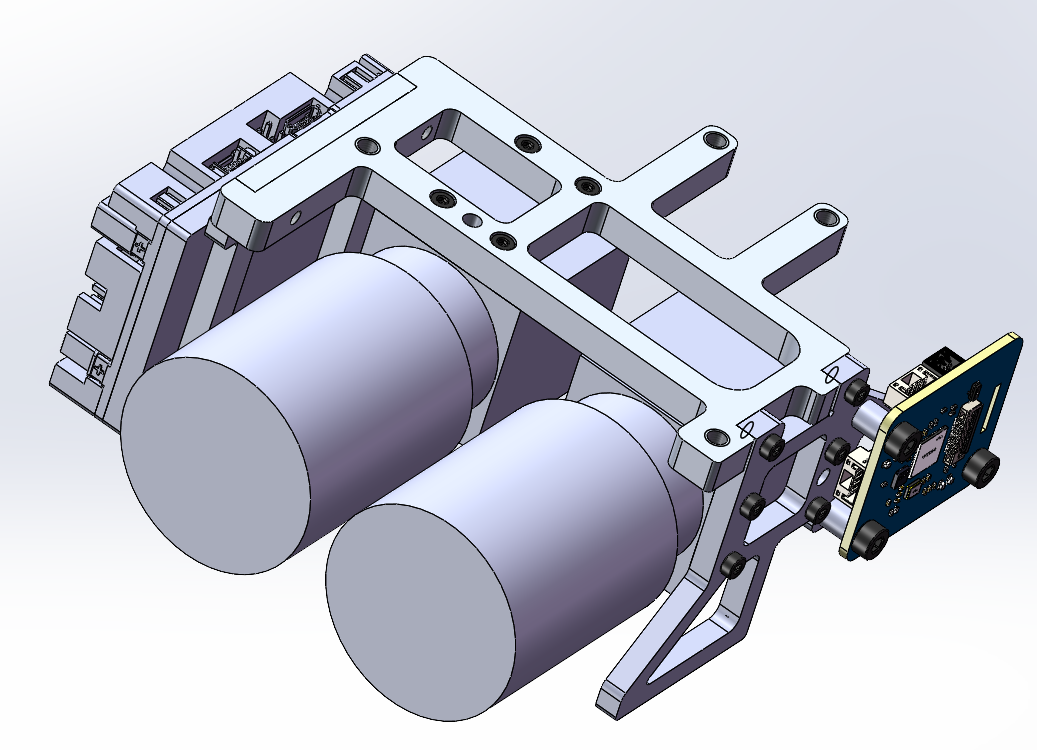
\includegraphics[width=0.8\columnwidth]{figure/4_详细设计/机械结构设计/双相机模块.png}
%     \caption{双相机模块}
%     \label{fig:双相机模块}
% \end{figure}

\paragraph{弹丸链路}

云台的链路设计部分首先需要明确云台Pitch轴的仰角与俯角，然后根据链路设计守则画草图，链路的转弯半径$24\mathrm{mm}$，再设计对应的活动挡边，关键是画好草图，否则就会在某些角度阻力增大导致弹丸运行不顺畅。

今年在云台链路方面进行了一项尝试：将Yaw轴与Pitch轴的转轴设计为同轴，以期获得更优的云台运动学特性。该方案虽然最终未在赛场上应用，但验证了设计思路的可行性。此外，在链路上涂抹了干性润滑油，有效减小了弹链阻力，提升了供弹流畅性。

Pitch轴采用四边形连杆传动，设计时注意压力角不能太小否则电机带不动，而且尽量设计成平行四边形连杆传动，使传力更均匀。

\paragraph{拨盘}

拨盘采用2006电机驱动，虽然有弹丸卡挡边等问题但性能稳定，能满足发射需求。拨盘位于云台架上方，通过波纹管与弹仓连接，负责将弹仓中的弹丸逐颗送入链路。

\paragraph{云台架}

云台架是连接机身与云台的部分，整个云台通过它吊装固定在机身下中心板上。由于云台需要向上仰角以实现近距离击打能量机关，为了防止弹丸发射弹道与桨保干涉，云台架设计得较长，我们称之为"长脖子"。

云台架采用三块厚碳板形成方形结构来吊装云台，能抵抗扭转与横向位移，大大增加了云台的稳定性，有效减小因为云台运动产生的晃动与形变。拨盘下沉到云台上方，用单独一层碳板固定拨盘与直角链路，再用波纹管连接拨盘与弹仓，消除了长段竖直链路带来的阻力问题。

% 图片占位：云台架结构图
% \begin{figure}[hbt!]
%     \centering
%     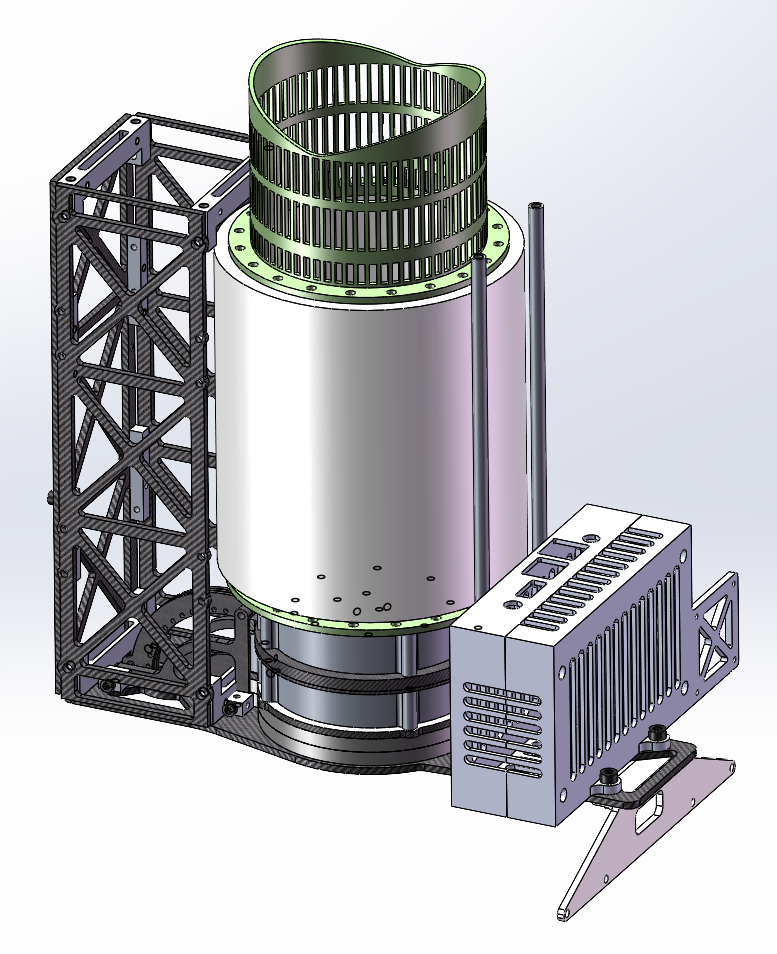
\includegraphics[width=0.8\columnwidth]{figure/4_详细设计/机械结构设计/云台架.png}
%     \caption{云台架（长脖子）结构}
%     \label{fig:云台架}
% \end{figure}

\paragraph{发射机构}

17mm小弹丸是依靠一对摩擦轮的旋转发射出去，而单发限位是发射机构中非常重要的结构。今年继续采用轴承式单发限位方案，通过在起始件上加一对U型轴承来限制预制位弹丸的活动。轴承是固定的，不会像拉簧一样反复入侵链路中，所以不会影响发射散度，而且轴承能够使每个出去的弹丸都在固定位置起到定心效果，提升发射精度。

今年发射机构的核心改动是将摩擦轮电机从M3508更换为M2006。M2006电机体积更小、重量更轻，且扭矩特性更适合摩擦轮发射场景。经过实际测试，更换后的发射散度得到了显著改善，达到了非常理想的效果。

轴承间距是影响发射性能的关键参数。今年对轴承间距进行了额外的测试优化，通过制作demo反复测试，确定了最优间距，既保证单发限位效果，又确保拨盘能顺畅转动。轴承的安装位置在摩擦轮之后，注意不与摩擦轮发射干涉。

% 图片占位：发射机构图
% \begin{figure}[hbt!]
%     \centering
%     \includegraphics[width=0.8\columnwidth]{figure/4_详细设计/机械结构设计/发射机构.png}
%     \caption{发射机构}
%     \label{fig:发射机构}
% \end{figure}
